% arara: xelatex
% arara: xelatex
% arara: xelatex


% options:
% thesis=B bachelor's thesis
% thesis=M master's thesis
% czech thesis in Czech language
% english thesis in English language
% hidelinks remove colour boxes around hyperlinks

\documentclass[thesis=B,english]{FITthesis}[2019/03/21]

\usepackage{todonotes}

%\usepackage[utf8]{inputenc} % LaTeX source encoded as UTF-8
% \usepackage[latin2]{inputenc} % LaTeX source encoded as ISO-8859-2
% \usepackage[cp1250]{inputenc} % LaTeX source encoded as Windows-1250

% \usepackage{subfig} %subfigures
% \usepackage{amsmath} %advanced maths
% \usepackage{amssymb} %additional math symbols

\usepackage{dirtree} %directory tree visualisation

% % list of acronyms
% \usepackage[acronym,nonumberlist,toc,numberedsection=autolabel]{glossaries}
% \iflanguage{czech}{\renewcommand*{\acronymname}{Seznam pou{\v z}it{\' y}ch zkratek}}{}
% \makeglossaries

% % % % % % % % % % % % % % % % % % % % % % % % % % % % % % 
% EDIT THIS
% % % % % % % % % % % % % % % % % % % % % % % % % % % % % % 

\department{Department of Software Engineering}
\title{Analysis of an IoT solution for assessment of physical difficulty of tourist tracks using smart wearables}
\authorGN{Zuzana} %author's given name/names
\authorFN{Václaviková} %author's surname
\author{Zuzana Václaviková} %author's name without academic degrees
\authorWithDegrees{Zuzana Václaviková} %author's name with academic degrees
\supervisor{Ing. Jan Krákora, PhD.}
\acknowledgements{THANKS (remove entirely in case you do not with to thank anyone)}
\abstractEN{Summarize the contents and contribution of your work in a few sentences in English language.}
\abstractCS{V n{\v e}kolika v{\v e}t{\' a}ch shr{\v n}te obsah a p{\v r}{\' i}nos t{\' e}to pr{\' a}ce v {\v c}esk{\' e}m jazyce.}
\placeForDeclarationOfAuthenticity{Prague}
\keywordsEN{Internet of Things, hiking track difficulty, activity tracking, heart rate monitoring, physical fitness assessment, smart wearables, software analysis, user experience}
\keywordsCS{Internet vecí, náročnosť turistickej trasy, sledovanie fyzickej aktivity, meranie tepu srdca, posudzovanie telesnej kondície, nositeľná elektronika, softvérová analýza, užívateľské skúsenosti}
\declarationOfAuthenticityOption{1} %select as appropriate, according to the desired license (integer 1-6)
% \website{http://site.example/thesis} %optional thesis URL

\graphicspath{ {./Images/} }

\begin{document}

% \newacronym{CVUT}{{\v C}VUT}{{\v C}esk{\' e} vysok{\' e} u{\v c}en{\' i} technick{\' e} v Praze}
% \newacronym{FIT}{FIT}{Fakulta informa{\v c}n{\' i}ch technologi{\' i}}


\setsecnumdepth{part}
\chapter{Task - temporary chapter}
\linebreak
Analysis of an IoT solution for assessment of tourist track physical difficulty

The aim of this thesis is to analyse, design and implement a proof-of-concept \todo{maybe change the way the acronyms are introduced?} (PoC) Internet-of-Things (IoT) solution for tourist track difficulty estimation.
Using a mobile application, the user shall be able to select a track and assess how difficult the specific part of the track will be for them, based on data collected from similarly fit users.
\begin{itemize}
    \item Analyse and compare similar existing solutions.
    \item Analyse and design an IoT solution for data processing.
    \item Design a mobile application for data visualization and track selection.
    \item Create a PoC of the IoT platform and of the mobile application.
    \item Collect raw data from smart watch heart rate sensors and smart phone GPS locators and propose relevant statistics to process this data.
\end{itemize}

\chapter{Aims}
The aim of this thesis is to analyse and design the functionality \todo{reword} of an IoT solution for assessment of tourist track difficulty, based on the individual's fitness.

In the theoretical chapters I will analyse existing applications in the domain of fitness trackers and e-health, assess the importance of specific features to the application's main usecases
and apply the results of this research to my own approach when determining the requirements for the system.
Based on these requirements, I will design the front-end of a mobile application for track selection and data visualization.
I will also design the overall architecture of the PoC solution.

In the practical part of the thesis I will focus on implementing a PoC of the designed solution - a mobile phone application for data collection and a platform for data receiving, with emphasis on usage of relevant data science methods. \todo{reword}

\chapter{Introduction}
With the increasing popularity of smart wearables in the general public, a growing number of people have been able to benefit from adjustments in their behaviour according to the way their data gets processed and fed back to them.
Runners can barely imagine not checking how fast and how efficiently they just ran their daily track or how much they have improved over the last month,
people with sedentary jobs attempt to keep their daily step count above a currently recommended number,
masses of people have been saving up for the Apple Watch 5~\cite{AppleWatch5} in spite of the ECG health monitor being virtually unnecessary for those not at risk of cardiac disease~\cite{ecg-screening}, etc.

All of this data is collected from a variety of devices, such as smartwatches, textiles with integrated sensors, jewelry, or more invasive ones such as implants or tattoos, all of which are meant to be worn on the user's body and which measure and send data for analysis - hence the name \textit{wearable technology}, or \textit{smartwear}~\cite{what-is-wearable-tech}.

Thanks to the data collected from these devices, the users have been keeping track of their health and fitness, setting goals for themselves and tracking personal achievements.
However, all of this is related to the past of each individual user, while the true potential of smartwear lies in collecting data from thousands of people,
finding patterns and correlations in large datasets and using the results to increase precision and improve upon whatever the data is being used for by the virtue of prediction.

That being said, the result of this thesis will be a design for an IoT solution, mainly to be used by hikers who want to not only pick a track on a map and see how long it is going to take them to get from point A to point B (which generally isn't tailored to the individual's fitness and often doesn't account for the possible rapid changes in the track's elevation profile),
but also an objective difficulty level of particular sections of said track, which may have additional benefits for people with cardiac issues or those trying to lose weight, who are interested in some more detailed insight into the exertion induced by the track in order to keep their heart rate in a specific range.
All of this will be available to the user before stepping foot on said track, thanks to the data collected from users with various fitness levels and their own history,
while the user's fitness will be presented more accurately as they continue to use the application.

I will study how fitness is assessed in regard to feasibility, availability for the general public, and precision, in order to provide fundamentals for further work.

Using methods of software engineering, I am going to analyse the use of wearable technology in existing applications and document the most common features as well as their outstanding traits and their use of IoT principles (or lack thereof).
Based on this analysis, I will pick the most relevant features to include in my design and extend them with features of my own devising, which will set my solution apart from existing software.

I will design and implement a PoC IoT solution -- a mobile application which will collect data from the smartwear sensor and an available GPS locator, along with a backend IoT platform to receive and process collected data, and the communication channels used between these two modules.
I will neither design nor implement a full-fledged IoT platform as that's not in the scope of this thesis.
I will design (not implement) the frontend mobile application for displaying of processed data, track selection with integrated maps and explore the necessary legal requirements for the use of such maps.

I will examine the use of different device types with heart rate sensors and choose one with which I will build my PoC.

I will collect and perform suitable operations on the collected data in order to visualize it.



\setsecnumdepth{all}
\chapter{Existing solutions}
There's a plethora of applications taking advantage of wearable tech, not all of them using the available bio sensors, ranging from basic real-time heart rate monitoring to progress tracking, to calorie measuring, and to social network sized fitness communities.

In this chapter I will research a few such applications, compare and rate them based on following criteria. \todo{add weight to individual points}
\begin{itemize}
    \item Use of IoT possibilities -- use of available sensors, data collection from the community,
    \item User fitness assessment -- how the user's fitness is assessed (attempt self-assessment, fill out a questionnaire, or take a physical test),
    \item Track difficulty assessment -- how the track's difficulty is assessed (user-reported, or calculated)
    \item Community -- built-in sharing options, possibility for interaction between users,
    \item Extra features -- interesting perks outside of the scope of my app,
    \item User-friendliness -- navigation around the mobile application - finding the general settings, creating and clearing a route, general user experience,
    \item Availability -- is the application or its parts free, paid or are there microtransactions,
    \item Cross-platform -- major operating systems supporting the mobile application and sensors, if any are used,
    \item Propriety -- whether the solution is open-source, closed-source or else.
\end{itemize}


\subsection{komoot}
The cross-platform application for outdoor track suggestion can also be used as a tour planner, a map and a navigation system.

\todo[color = green]{add numeric ratings}

\subsubsection*{Use of IoT possibilities}
Given its use of GPS sensors, komoot does qualify as a basic IoT system, however, it also relies heavily on user input for track rating.
The smart watch only gets used for displaying of routes and navigation, not taking any advantage of the available sensors.
\subsubsection*{User fitness assessment}
When a user is creating a route, they can set its difficulty as one of five levels, 
describing the user's self-reported physical fitness and their current taste for a challenge (or lack thereof): Couch Potato, Average, In Good Shape, Athletic, and Pro.
This parameter is considered when the app is generating a suitable route -- presumably by trying to adjust the elevation profile of the possible routes.
The user's real fitness is not taken into account.
\subsubsection*{Track difficulty assessment} 
Thanks to the maps provided by the OpenStreetMap, users are able to pick a starting point, a destination, as well as any number of waypoints in between for their route.
Once the route is chosen, the user can go through the route's stats - the estimated time it will take to get from start to finish, its length, the elevation profile (uphill, downhill, highest and lowest points, estimated average speed) and the surfaces and their use in proportion to the route's length.
All this information is delivered in easy-to-understand charts as well as interactive mappings -- using a slider, the user can see which stat applies in which part of the route.

\begin{figure}[h]
    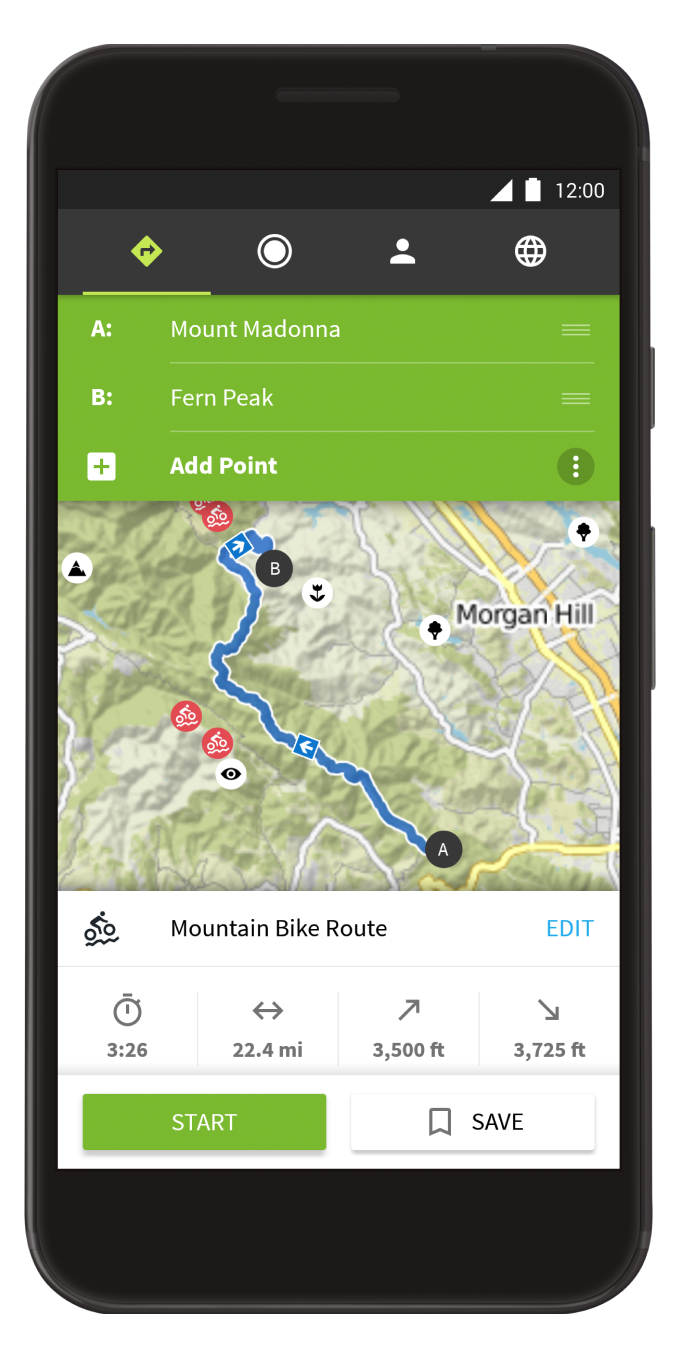
\includegraphics[width=\textwidth]{komoot-nav.png}
    \caption{Offline maps in the komoot app\cite{komoot-nav-img}}
\end{figure}

\begin{figure}[h]
    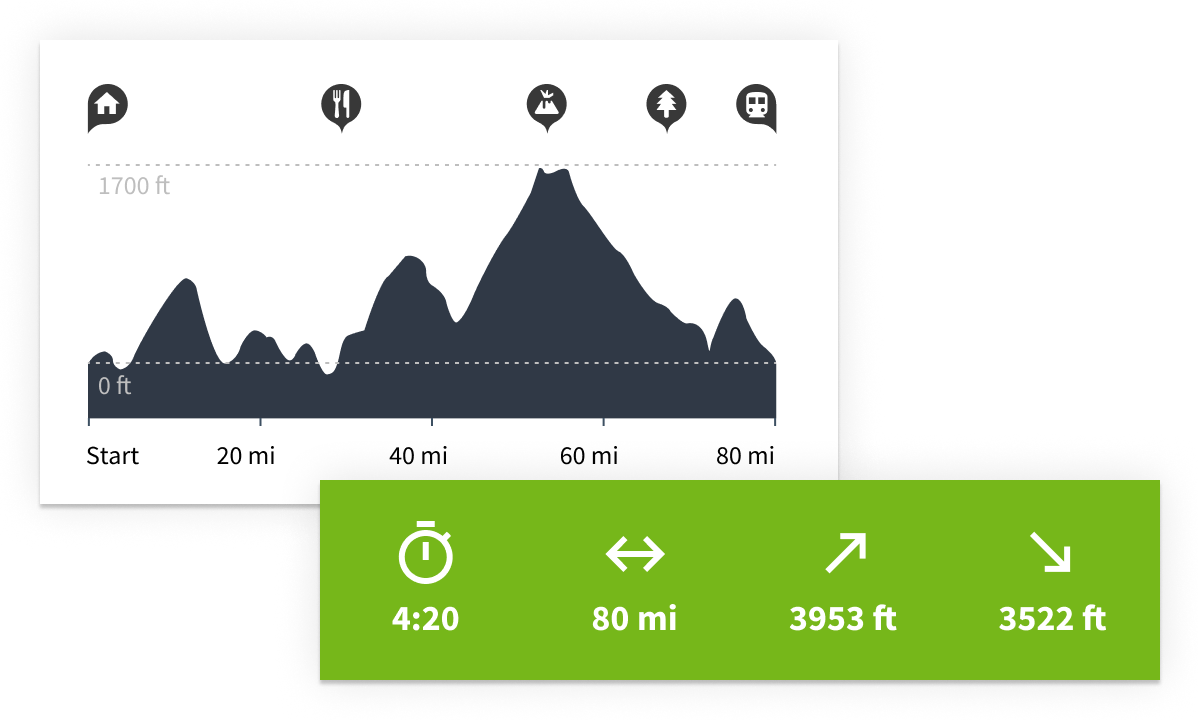
\includegraphics[width=\textwidth]{komoot-route-details.png}
    \caption{Route elevation profile\cite{komoot-route-details-img}}
\end{figure}

\begin{figure}[h]
    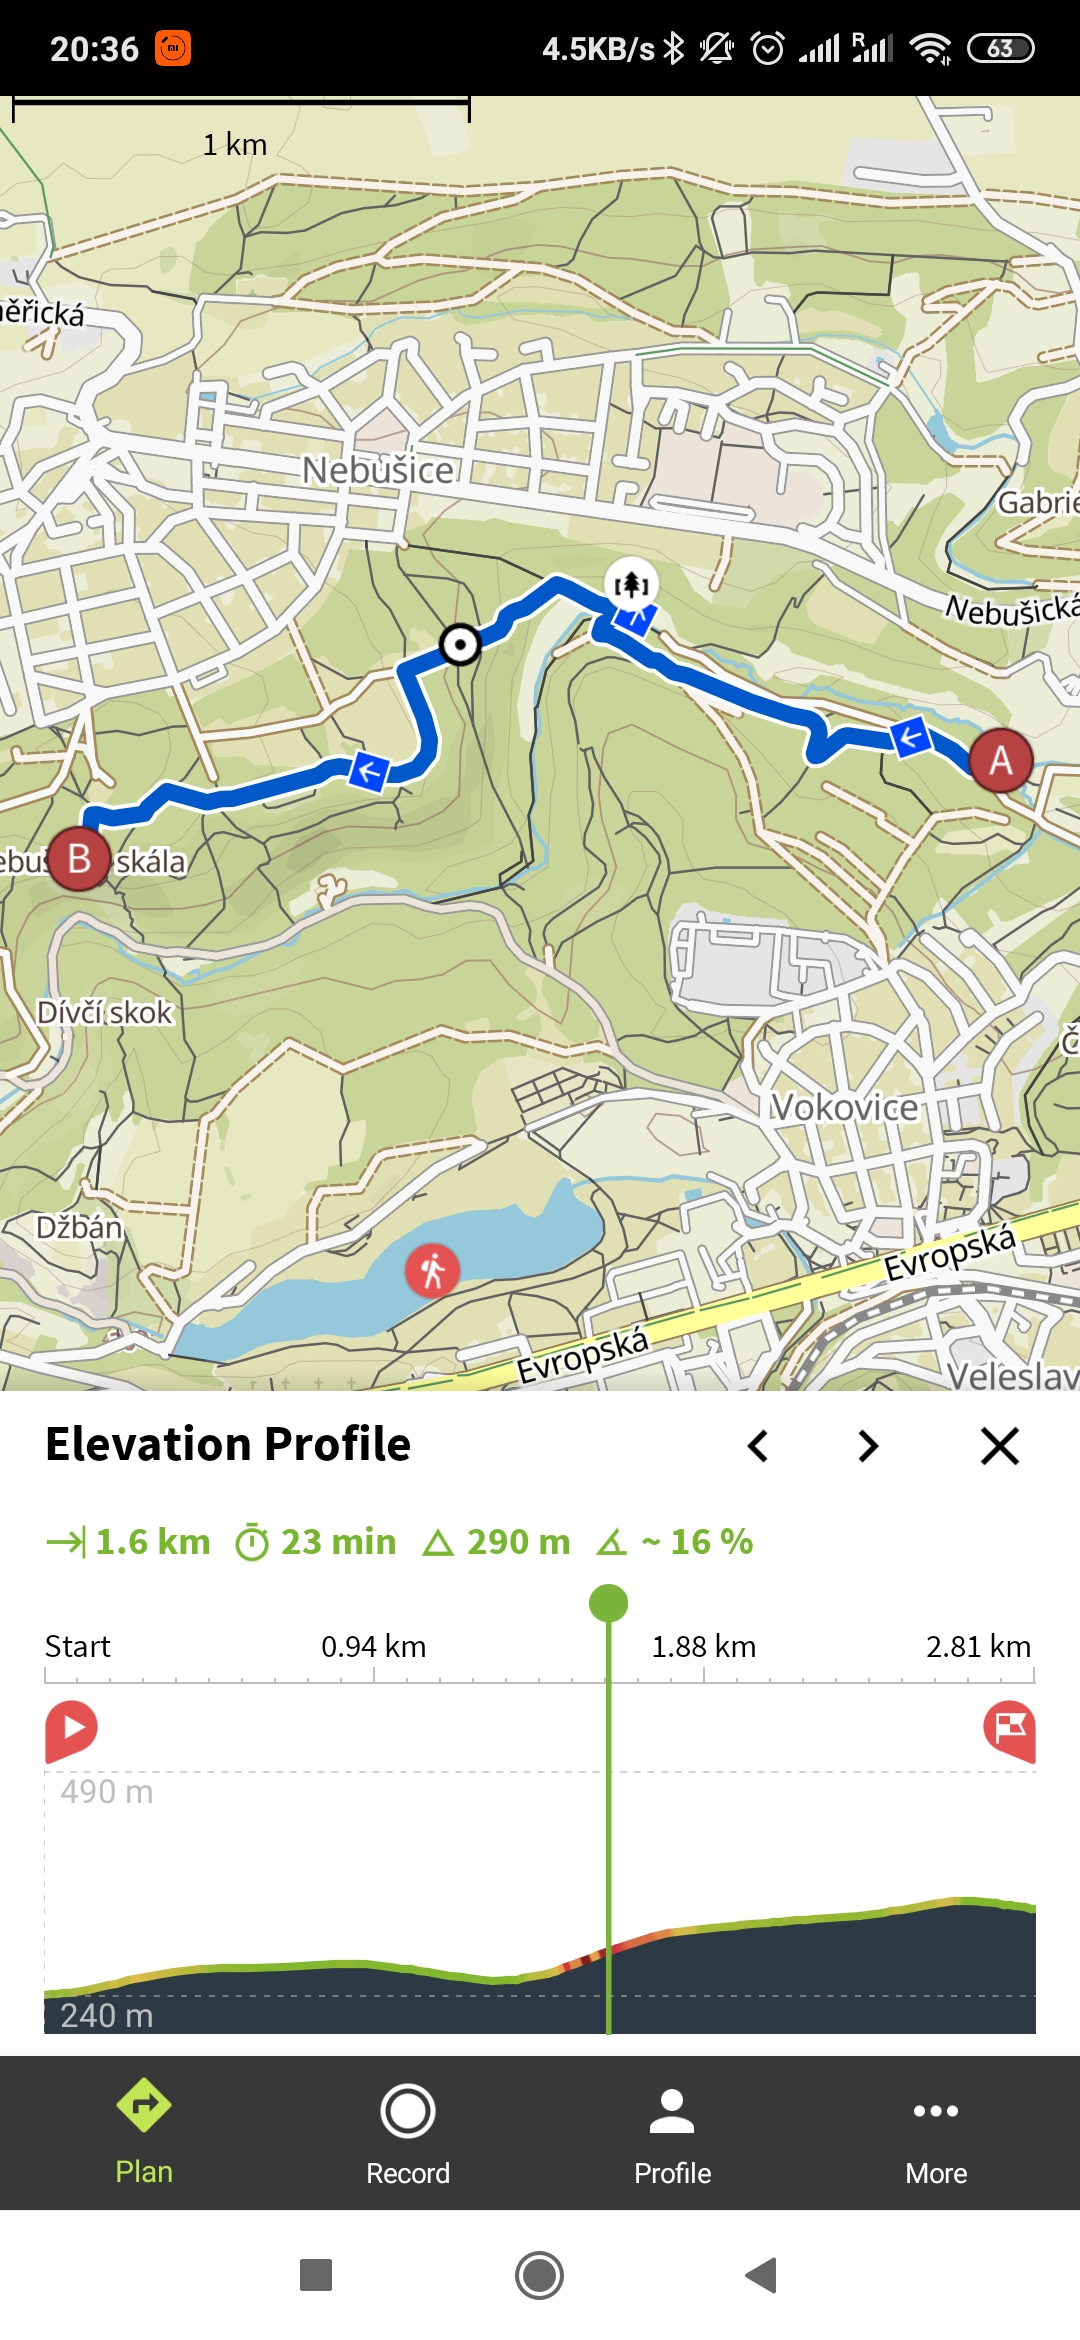
\includegraphics[width=\textwidth]{komoot-route-elevation-detail.jpg}
    \caption{Detailed view of the route's elevation\cite{komoot-route-elevation-detail-img}}
\end{figure}

\begin{figure}[h]
    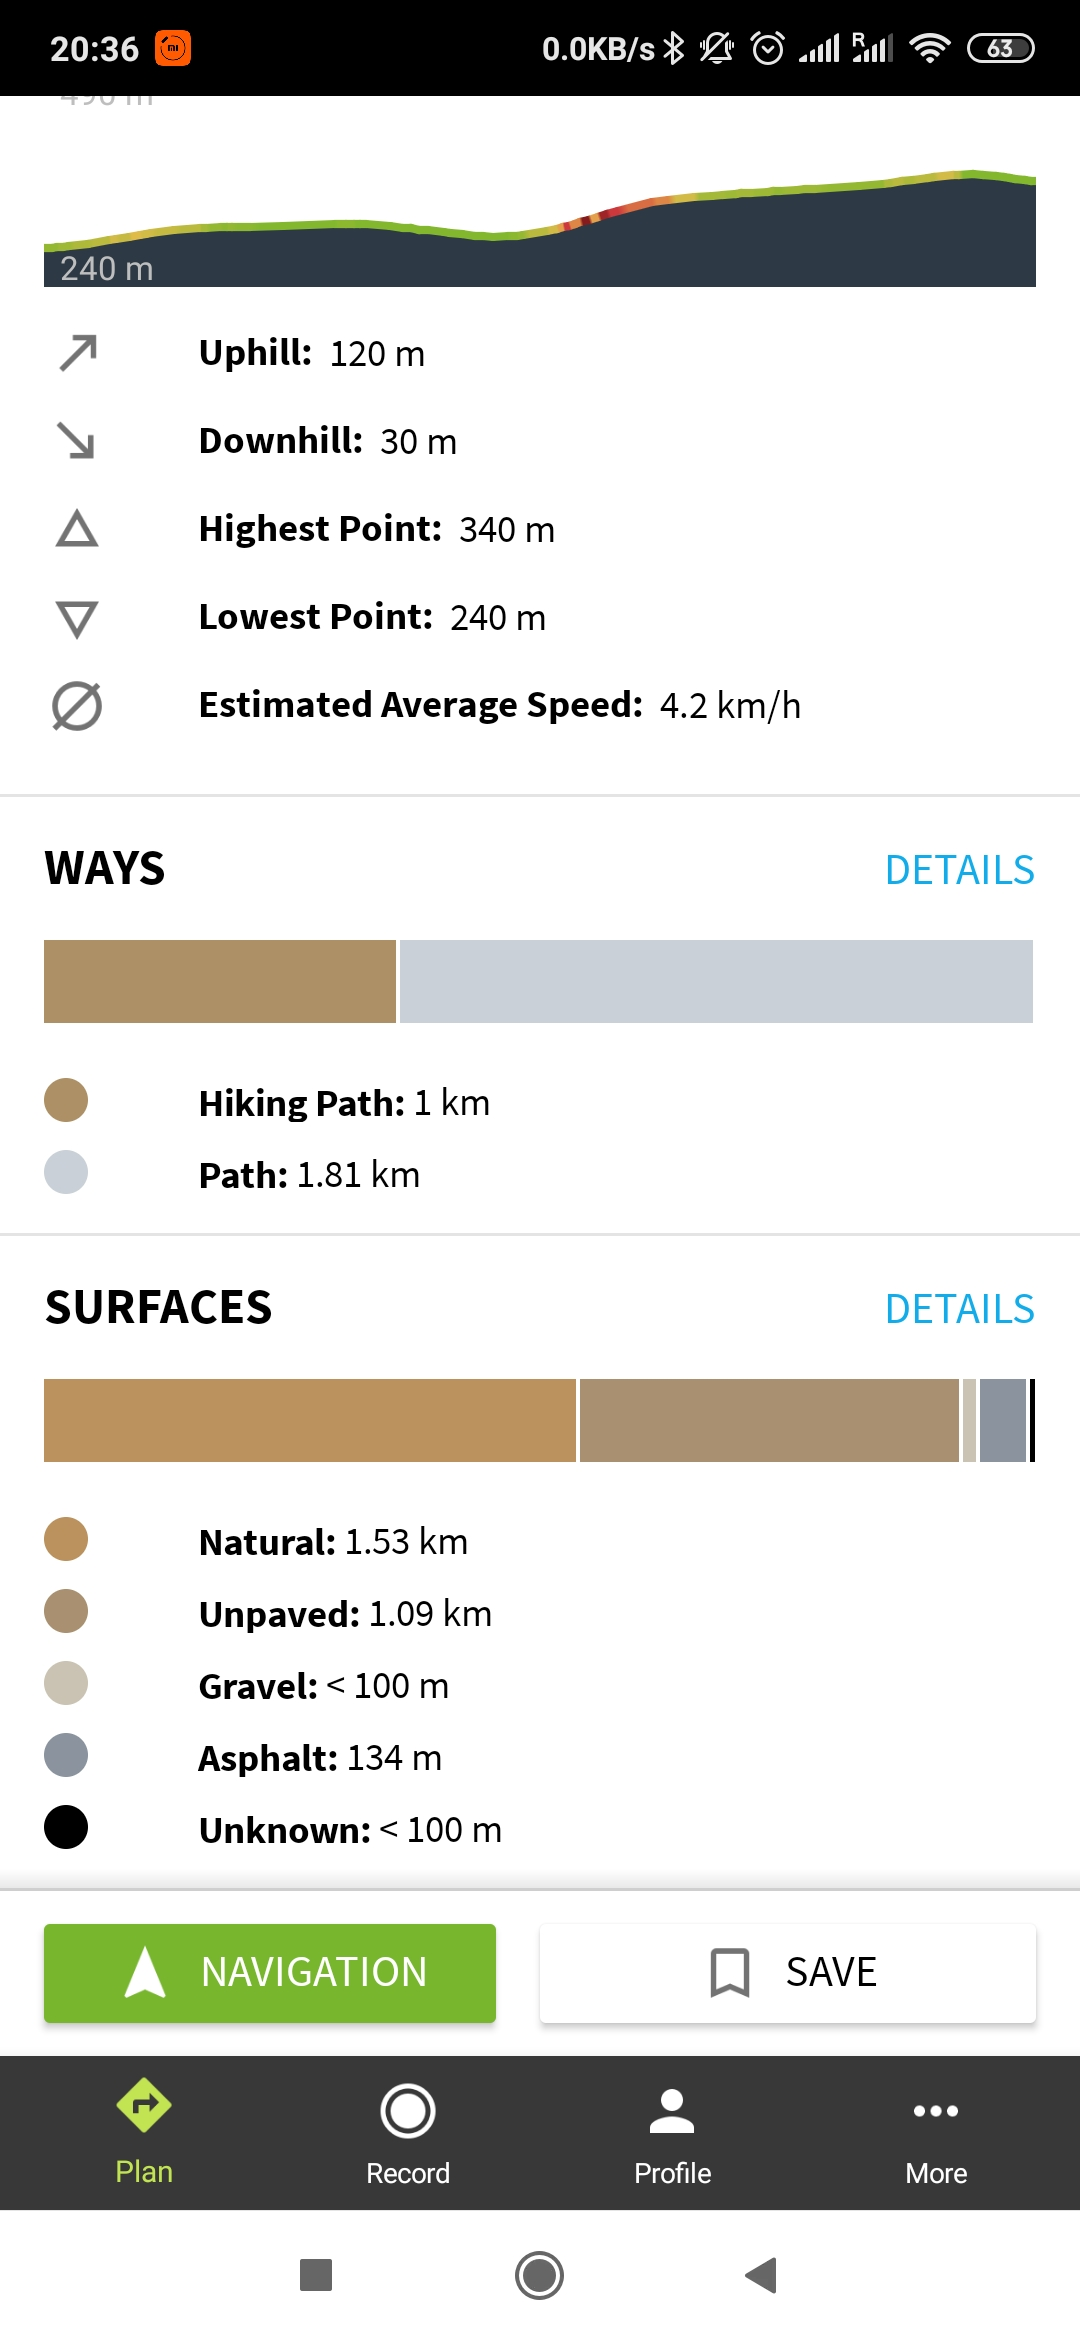
\includegraphics[width=\textwidth]{komoot-route-surface-detail.jpg}
    \caption{Overview of the route's surface. The detailed view is similar to the elevation detail.\cite{komoot-route-surface-overview-img}}
\end{figure}


\subsubsection*{Availability}
The region-based pricing model allows users who do not travel too much to use the app for free,
since the first region is provided at no cost.
In the other pricing options Single Region, Region Bundle and All Regions -- the price-performance ratio seems to grow at a reasonable scale.\todo[color = green]{anything to add?}
\subsubsection*{Community}
With features like sharing of routes users have taken, following of other users, upvoting and commenting on their posts, the mobile application integrates a full-fledged social network.
\subsubsection*{Extra features}

\subsubsection*{User-friendliness}
The navigation through the mobile app takes some time to get used to -- it took me a while to find the Settings after I didn't see them in the burger menu on the bottom navigation bar, which contained only the different pricing options.
Once I created a route, the information provided was well-delivered and easy to read, however, there was no obvious way of completely cancelling the chosen route and picking another one.
Instead, hiding in the Options of the route -- which at first I didn't even notice -- I found the "Reset route" option, which did just what I needed.
Overall, the app has some great parts and some not-so-great ones.
\subsubsection*{Cross-platform}
The system is fully integrated with the Apple Watch and Samsung gear, and -- at least limitedly -- supports a number of other brands of smart watches and other Bluetooth-enabled devices.
The mobile application runs both on iPhones and Android phones.
\subsubsection*{Propriety}
The system is not entirely open-source, as a few of their repositories are public, but the core components remain proprietary. \todo[color = green]{recheck}\todo[color = green]{cite https://github.com/komoot}

\subsubsection*{Overall evaluation}
While being rich with features, komoot doesn't base its functionality on objective data -- it's the users themselves who rate and recommend the specific routes,
an approach in its nature prone to error and with only limited ways of eliminating the human factor.

\subsection{endomondo}
https://www.endomondo.com/
\subsubsection*{Use of IoT possibilities} --
\subsubsection*{User fitness assessment} --
\subsubsection*{Availability} --
\subsubsection*{Community} -- 
\subsubsection*{Extra features} -- 
\subsubsection*{User-friendliness} -- 
\begin{figure}[h]
    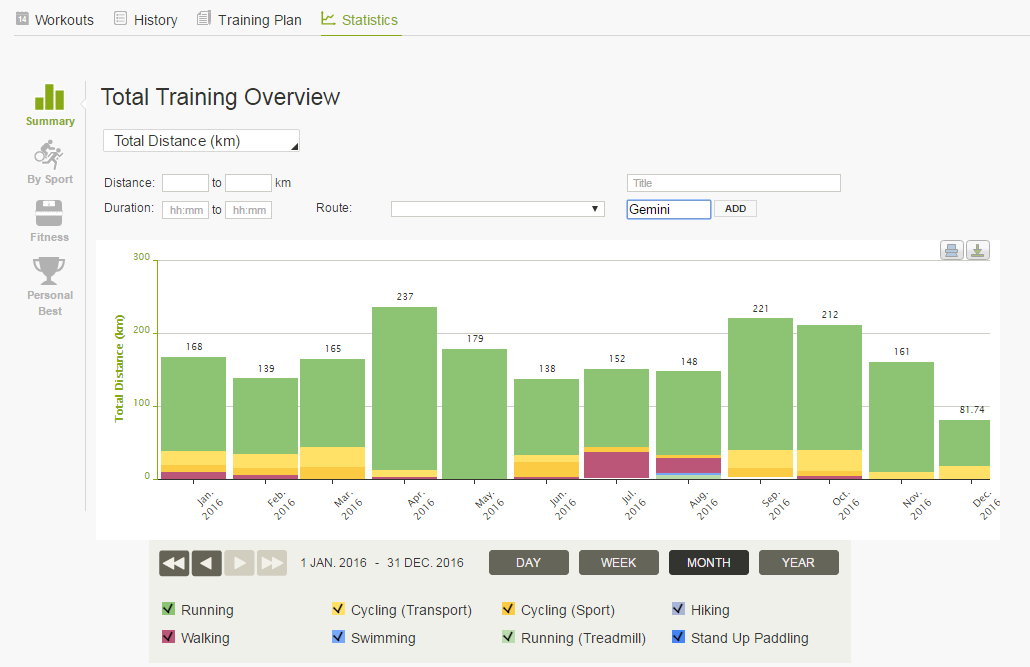
\includegraphics[width=\textwidth]{endomondo-history-example.png}
    \caption{endomondo history example\cite{endomondo-history-img}}
\end{figure}

\begin{figure}[h]
    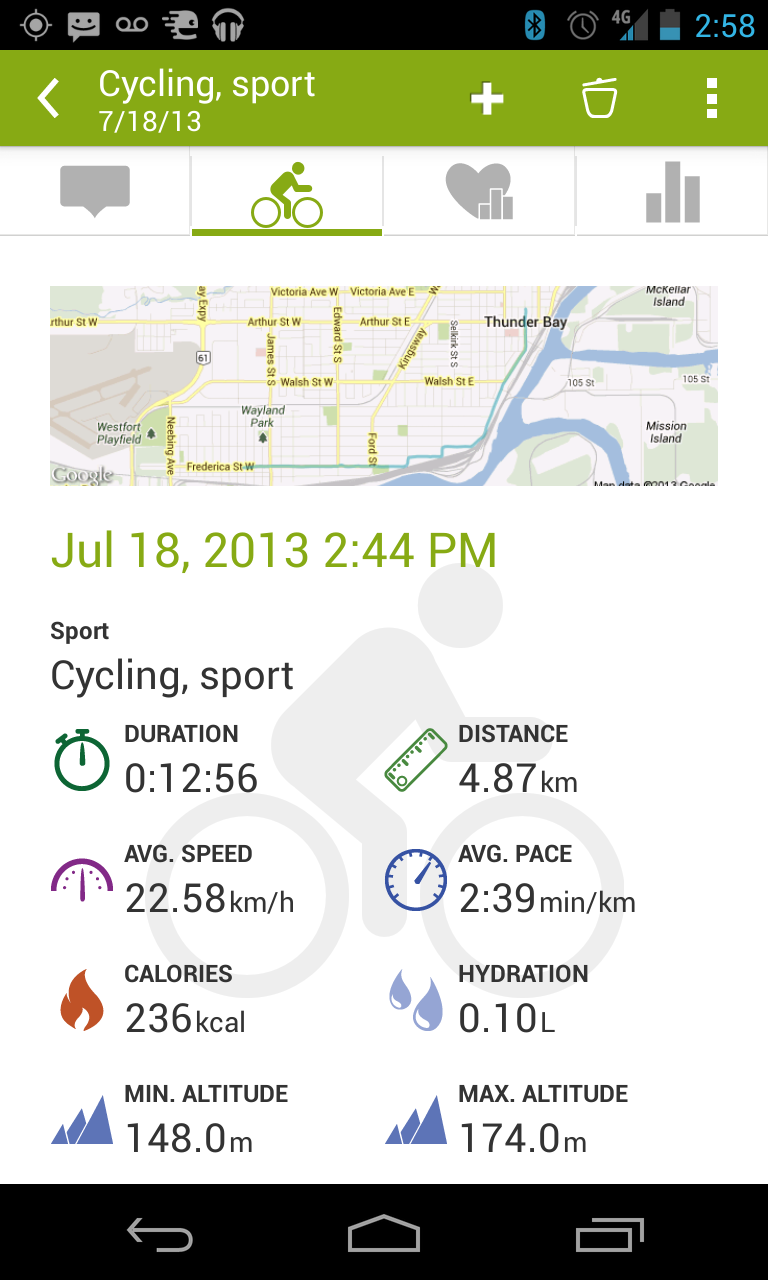
\includegraphics[width=\textwidth]{endomondo-bike-stats.png}
    \caption{Statistics of a biking trip on endomondo\cite{endomondo-bike-stats-img}}
\end{figure}

\subsubsection*{Cross-platform} -- 
\subsubsection*{Propriety} -- 
\subsubsection*{Overall evaluation}

\subsection{Strava}
https://www.strava.com/
\subsubsection*{Use of IoT possibilities} --
\subsubsection*{User fitness assessment} --
\subsubsection*{Availability} --
\subsubsection*{Community} -- 
\subsubsection*{Extra features} -- 
\subsubsection*{User-friendliness}
\begin{figure}[h]
    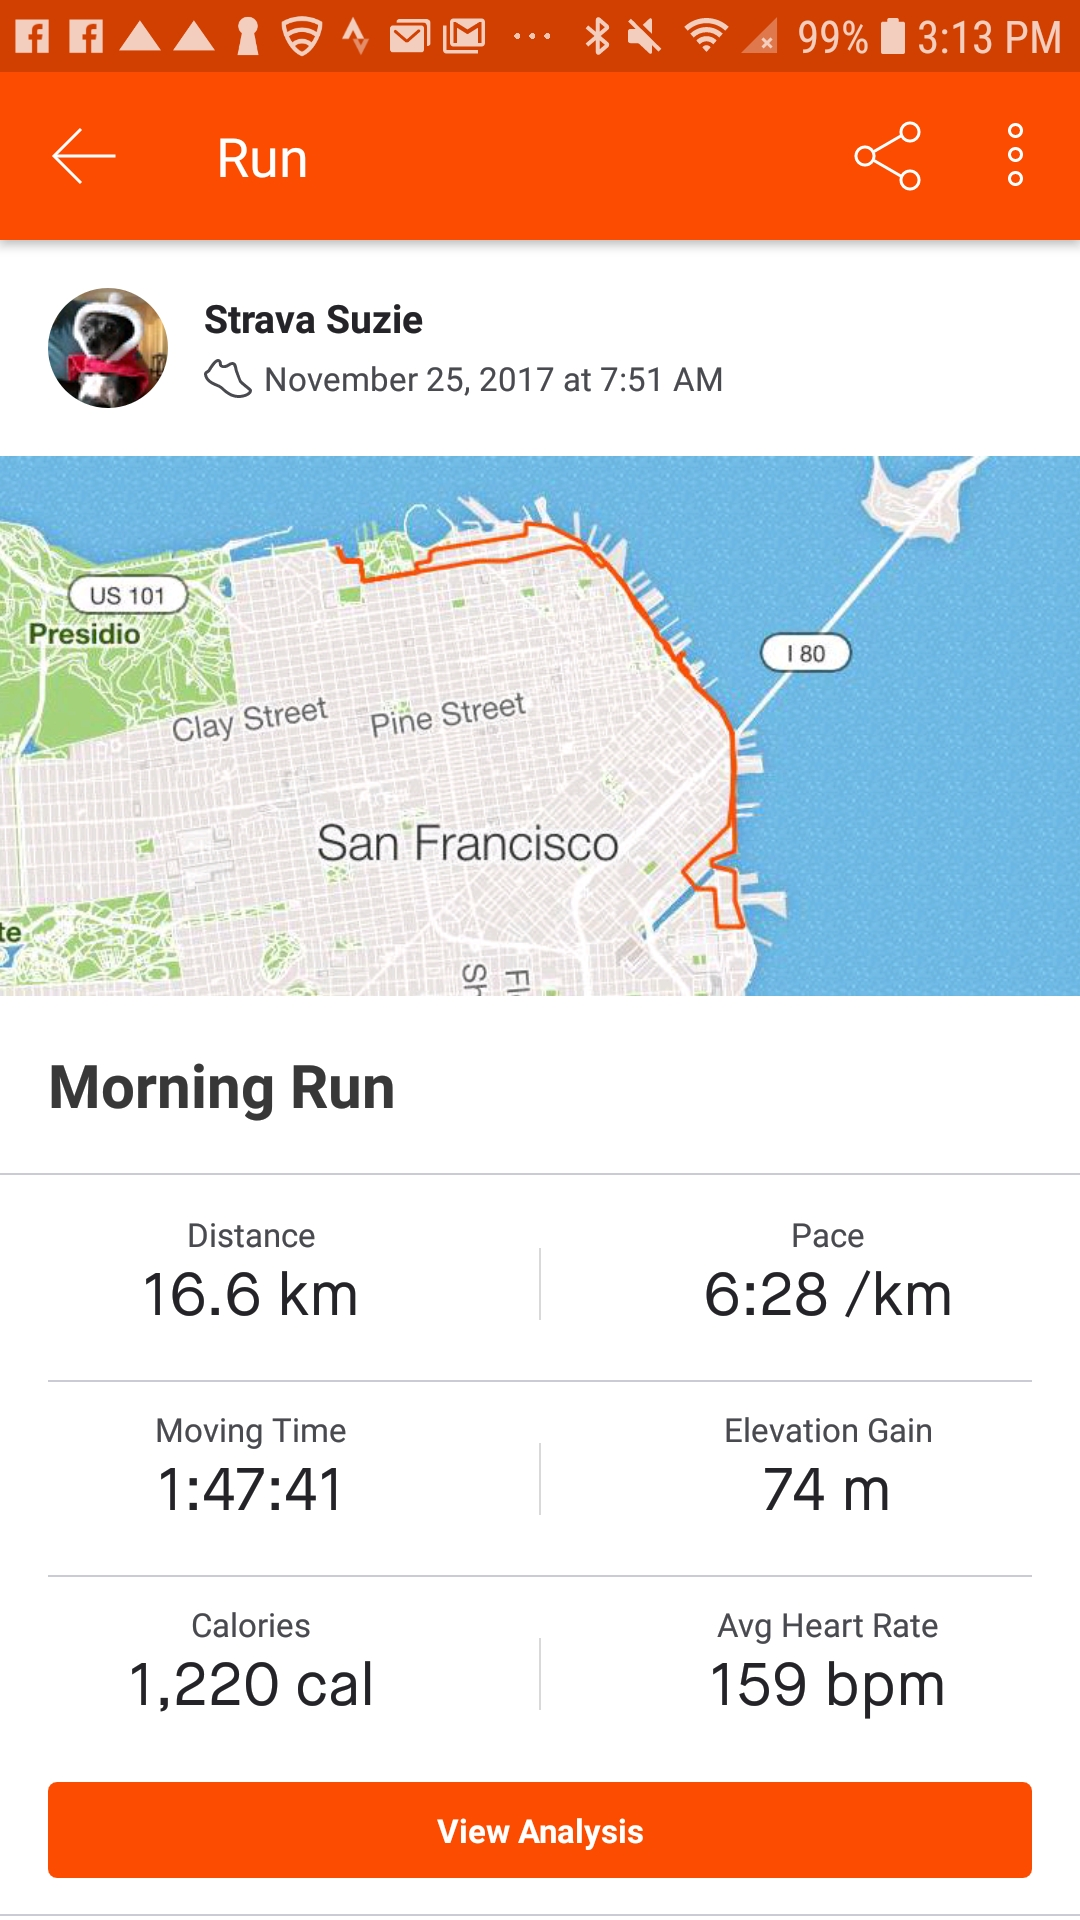
\includegraphics[width=\textwidth]{strava-morning-run-stats.jpg}
    \caption{Statistics of a run on strava\cite{strava-run-stats-img}}
\end{figure}
\subsubsection*{Cross-platform} -- 
\subsubsection*{Propriety} -- 
\subsubsection*{Overall evaluation}

\subsection{myFitnessPal}
https://www.myfitnesspal.com/
\subsubsection*{Use of IoT possibilities} --
\subsubsection*{User fitness assessment} --
\subsubsection*{Availability} --
\subsubsection*{Community} -- 
\subsubsection*{Extra features} -- 
\subsubsection*{User-friendliness} -- 

\begin{figure}[h]
    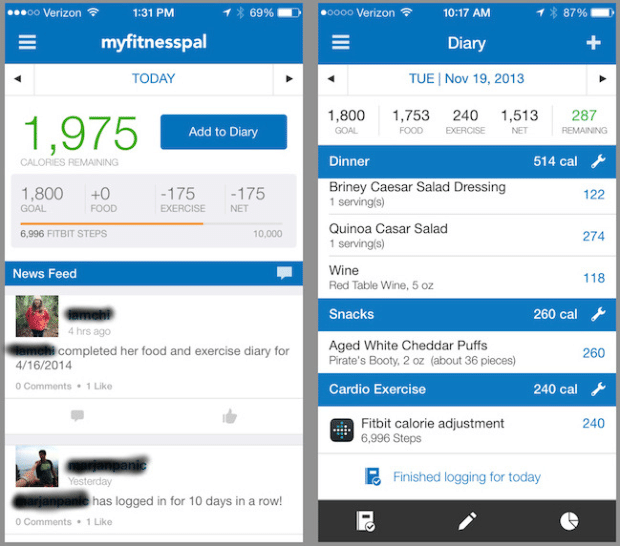
\includegraphics[width=\textwidth]{myfitnesspal-researchgate.png}
    \caption{myFitnessPal feed and diary entry\cite{MFP-diary-img}}
\end{figure}

\subsubsection*{Cross-platform} -- 
\subsubsection*{Propriety} -- 
\subsubsection*{Overall evaluation}

\subsection{Walk with Map My Walk}
https://www.mapmywalk.com/
\subsubsection*{Use of IoT possibilities} --
\subsubsection*{User fitness assessment} --
\subsubsection*{Availability} --
\subsubsection*{Community} -- 
\subsubsection*{Extra features} -- 
\subsubsection*{User-friendliness} -- 

\begin{figure}[h]
    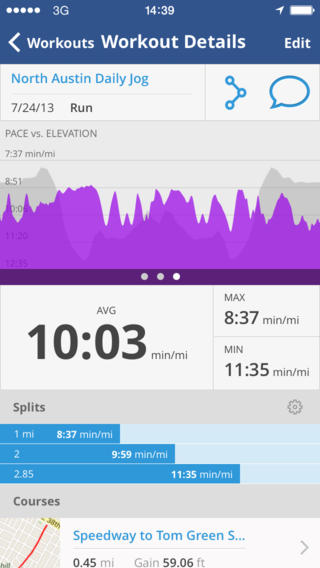
\includegraphics[width=\textwidth]{map-my-fitness-workout-details.jpg}
    \caption{Map my Fitness workout details\cite{map-my-walk-img}}
\end{figure}


\subsubsection*{Cross-platform} -- 
\subsubsection*{Propriety} -- 
\subsubsection*{Overall evaluation}

\subsection{Garmin Explore and Garmin Connect}
The vast ecosystem Garmin has created for their users is filled with an assortment of wearables, radars, smart lights, navigations, customized maps, and plenty more, providing features which are presented to the user via modular mobile apps.

Here I will analyse the Garmin Explore application, which is targeted at hikers, in tandem with Garmin Connect, which functions as a fitness tracker.

\subsubsection*{Use of IoT possibilities}
Most fitness-focused Garmin watches do have a heart rate sensor and all of them include a step counter, however, this data is never compared with that of other users, keeping focus on the user's activity history with no prediction.
\subsubsection*{User fitness assessment}
Some of the heart-rate-monitor enabled watches allow a user to set the zones in which they would like to keep their heart rate depending on the activity they choose to do. The standard zones are:
\textit{
\begin{itemize}
    \item Zone 1 (Warm Up) --
    Perceived exertion: Relaxed, easy pace, rhythmic breathing. Benefits: Beginning-level aerobic training, reduces stress.
    \item Zone 2 (Easy) --
    Perceived exertion: Comfortable pace, slightly deeper breathing, conversation possible. Benefits: Basic cardiovascular training, good recovery pace.
    \item Zone 3 (Aerobic) --
    Perceived exertion: Moderate pace, more difficult to hold conversation. Benefits: Improved aerobic capacity, optimal cardiovascular training.
    \item Zone 4 (Threshold) --
    Perceived exertion: Fast pace and a bit uncomfortable, breathing forceful. Benefits: Improved anaerobic capacity and threshold, improved speed.
    \item Zone 5 (Maximum) --
    Perceived exertion: Sprinting pace, unsustainable for long period of time, labored breathing. Benefits: Anaerobic and muscular endurance, increased power.\cite{garmin-heart-zones}
\end{itemize}
}

\begin{figure}[h]
    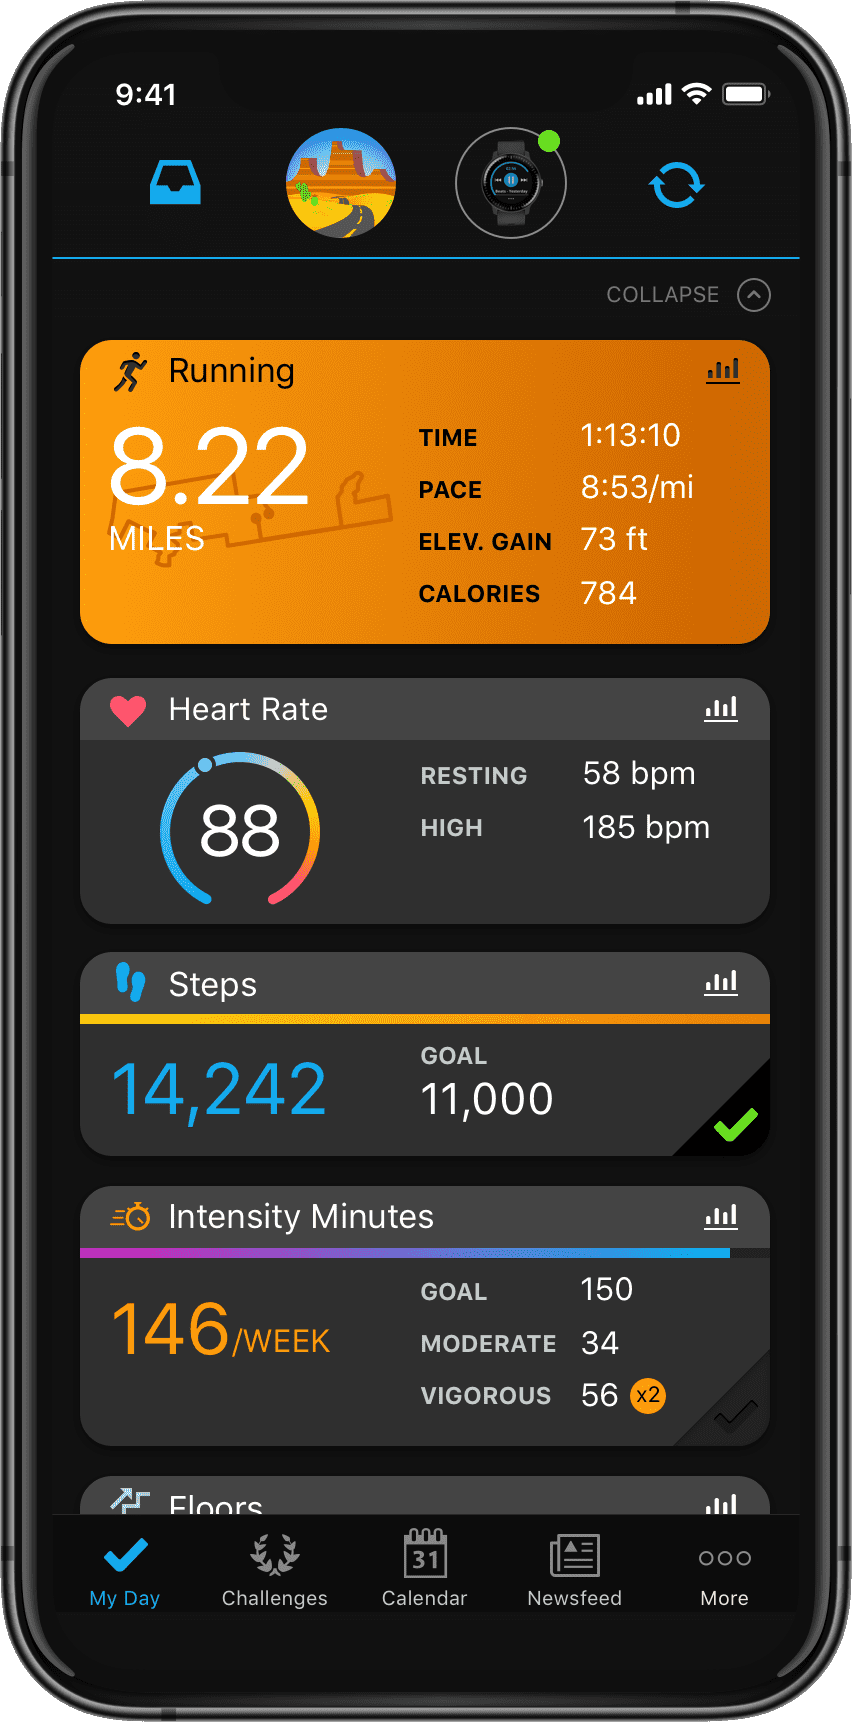
\includegraphics[width=\textwidth]{garmin-connect-myday-screen.png}
    \caption{My day - Garmin Connect's home screen displays statistics of the user's recent activity\cite{garmin-my-day-img}}
\end{figure}

\subsubsection*{Track difficulty assessment}

\subsubsection*{Availability}
In general, Garmin's pricing model relies on the user buying one of their high-end smartwatches, whereupon the rest of the components (apps, basic maps, support, etc.) are free, with some exceptions, such as advanced maps. 
The company's smartwatches are considered premium quality, with a wide price range - target groups include \textit{potential Rolex buyers}\cite{garmin-expensive} as well as ordinary users.\cite{garmin-watches-review}
\subsubsection*{Community}
The Connect application handles the data from the point of view of a fitness tracker, with social features like groups, competitions, likes, comments, and badges of accomplishment.\cite{garmin-connect}
\subsubsection*{Extra features} -- 
\subsubsection*{User-friendliness}

\subsubsection*{Cross-platform}
All of Garmin's applications can be installed both on Android and iPhone.
However, they can only be paired with watches inside Garmin's ecosystem, which is a drawback for users who already own a smartwatch.
\subsubsection*{Propriety}
Some of the Garmin applications are completely open-source, either due to the software that they are derived from, or simply to provide the general public with opportunity to customize their Garmin experience.\cite{garmin-open-source}\cite{garmin-connect-github-repos}
These apps are mostly concerned with map handling, navigation and sound codecs, but also include some bits of functionality like widgets, low power watch apps and others.

While some of this code may be used in the Explore or Connect applications, these repositories don't contain their core functionality.

\subsubsection*{Overall evaluation}
As a fitness tracker, Garmin Connect can definitely be considered acceptable...

\chapter{Requirements}
\linebreak
Based on the analysis of existing solutions, I will now describe the most important features that should be provided by my software.

I decided to construe the user-focused features (usually functional requirements) as one would in a real-life agile project, as this is in my experience more straightforward and easier to alter when necessary than flooding the reader -- for example, a developer -- with a long list of elaborate use cases right away.
The discussions that took place before reaching a specific conclusion should be well documented -- brief enough and detailed enough at the same time to provide good value after a quick read.
If the reader has access to a good transcript of these discussions, it is less likely that they will misunderstand the requested functionality;
in the best case scenario, if the reader is the potential developer, they are an active part in those discussions, so they have a substantial impact on the outcome, thus diminishing the `coding monkey' phenomenon.

The top-down approach of the agile methodology which is perhaps the most common and natural to grasp is creating epics, decomposing them into user stories, and with good knowledge of the project's architecture and after due consideration, technical subtasks in an issue tracker of choice.

Epics are complex, high-level characterizations of desired functionality, which usually take longer to deliver than a few weeks.
An epic is usually comprised of a description and multiple user stories, which cover the extent of the epic in higher granularity.
Once all the stories are delivered, the whole epic is considered finished.
Epics are sometimes formulated using the same format as user stories.

User stories (US) are short, simple descriptions of a feature told from the perspective of the person who desires the new functionality, usually a user of the system.\cite{user-story-definition}
Often they are written in simple, non-technical language, as most systems don't have tech-savvy users.
The typical template for a user story is:
\textit{As a < type of user >, I want < some goal > so that < some reason >.}\cite{user-story-definition}
Sometimes the US's aren't technical per se, but request deeper analysis and block further progress on the epic.

The main focus of this chapter will be to document my internal discussions, occassionally consulted with developer friends. \todo{cite? delete completely?}
I will always start with a high-level description of the requested feature formulated as an epic or a user story and elaborate on its details incrementally.
Since a part of this thesis will focus on implementing a proof of concept, some of the most imperative stories will also be fully processed and finished.

Features
\begin{itemize}
    \item F -- Track selection
    \item F -- Heart rate monitoring
    \item F -- Objective user fitness assessment
    \item F -- Calculation of selected track's difficulty relative to user's fitness
    \item F -- Map integration
    \item F -- Track details display
    \item F -- Track segment details display
    \item F -- How long the track will take
    \item F -- History of tracks the user has chosen
    \item F -- Mood of user after finishing of track
    \item F -- Option to insert fitness level manually instead of using the built-in calculator (maybe the user has done a lab test)
\end{itemize}

\subsection*{E01 -- Heart rate monitoring}
The application should monitor a user's heart rate inobtrusively and reliably.

The user needs a method for getting their data to the mobile application and then to the backend, do it comfortably, preferably without need for direct user-computer interaction.

\subsection*{E01-US01 -- Choose and integrate a wearable}
As an APP user, I want my heart rate-enabled wearable to work with the APP, so that I don't have to buy a new one.

Based on the analysis of existing applications, the most often used type of wearable tech are smart watches.
While most applications support other devices, such as chest straps, watches are the most convenient and wide-spread gadgets to be used by the general public.
There are a few quite popular smart watch vendors, most of whom have proprietary protocols of communicating with the system for data processing.\todo{recheck}
At the time of writing, however, Garmin seems like the most popular option, in spite of being more than a little costly.

It will be more difficult to integrate some devices.
Some vendors don't disclose their devices' API, or the API's documentation is only in Chinese and available to for use exclusively by partners of the given vendor,
some don't get paired with the phone itself but with a vendor app using server based pairing (such as the Xiaomi Mi Band 4 I initially intended to use) and there is no easy or straight-forward way to get the data.
For example, getting data from the Mi Band 4 would require root access to the user's phone\cite{miband4-server-based}, which is just not an option for a normal user.
Therefore I recommend limiting the supported devices to those that do not use server based pairing, as this would cover most of the currently available gadgets.

For my PoC in this thesis, I chose the XXXXXXXXX.\todo{add what and why}

\subsection*{E01-US02 -- Manage devices paired with the APP}
As an APP user, I want to pair and unpair my wearables with the APP, so that the APP can use the data of all devices that I currently own.

The user should be able to pair and unpair any number of wearables they choose.
The app should provide the user with the list of the phone's paired devices, so that they can choose their fitness gadgets.

Restrictions on which data gets processed if multiple devices are measuring the same biometric is described in E01-US03.

\subsection*{E01-US03 -- Activate a device}
As an APP user, I want to mark a wearable I'm using as active, so that only its data is relevant to the statistics.

The user should be able to activate a device they want to use for monitoring of current activity or activity in the near future.
Only one device should be active at a time, so if device A is marked as active and user tries to activate device B, device A gets deactivated before device B is marked as active.

\subsection*{E02 -- Objective user fitness assessment}
As an APP user, I want my fitness to be assessed, so that I can get relevant estimations of track difficulty.

Having analyzed the conventional ways of user fitness assessment in a previous chapter, the application should allow a user to use one of multiple ways to get their fitness level.
The outcome of the assessment should be the individual's VO2 max index and their heart rate zones -- so that if they need to maintain their heart rate in a specific range, they can cross-reference it with the exhaustion they perceive and learn to recognize when they are in the desired zone.

If the user has no physical impairments, they can have their HR max assessed by a simple age-based formula, such as the one developed by Nes et al. (see chapter on fitness assessment).

Users with physical impairments could self-evaluate how much their condition affects their fitness, and based on this their HR max can be set by using one of the standard formulas and subtracting a smaller or larger number of beats per minute (further research needs to be done on how many beats this should be).
This self-assessed value should be corrected as more data is available about the user.

As far as objective assessment, I see plenty of potential for the use of neural networks.
The networks can learn from the data collected from a good number of users over a longer period, and then categorize the new users into fitness groups based on this data, which will then be used to predict the users' future hikes.

\subsection*{E02-US01 -- Implement support for VO2 max tests}
As an APP user, I want to be able to take a guided test of my fitness in the APP, so that I don't have to look for tests elsewhere.

The APP should implement a guide to multiple tests of VO2 max, with instructions on what they should do, and signals to direct the user while taking the test.
The instructions should also contain a description of the signals the user will receive.
The initial instructions should definitely be textual and possibly audible, so that the user understands the aim of the test before taking it.
During the test, a watch vibration should alert the user about an incoming signal which will be displayed on the watch.
This signal would contain directions like 'Turn in N seconds' where N is a countdown to 'Turn now!'.
When no signals are occupying the device's screen, there should be pep talks like 'Keep going!' and 'Great job!'.
At all times during the test, there should be the test status on the device's screen: remaining time, distance walked, and any other metric relevant to the test.

As it is the most accurate of the more feasible tests, the application should encourage the user to take the 6-Minute Walking Test, and let them take it using the app in both 15- and 30-metre-long variations.
In order to calculate VO2 max, the APP can use Mänttäri's formulas.

\subsection*{E02-US02 -- Implement support for HR max tests}
As an APP user, I want to be able to take a guided test to find my heart rate zones in the APP, so that I don't have to look for tests elsewhere and get as accurate heart rate zones as possible.

The implementation should be similar to VO2 max tests; in fact, if possible, both metrics should be measured by a single test if possible.

\subsection*{E02-US03 -- Allow other input of biometric values}
As an APP user who has done lab fitness tests, I want the APP to use these values instead of doing the APP's tests, so that I don't have to take fitness tests that are most probably less accurate than what I know.

If a public universal database with all people's medical data existed, it would make sense to get the necessary information directly via an API.
In the real world, however, we will let the user enter their biometric data manually.
The APP definitely needs easily available data like age, sex and weight.
Then it should be possible to either take tests on or manually enter the VO2 max, resting heart rate and maximum heart rate.


\chapter{Fitness assessment}
Since the platform should estimate how a user will be affected by a hike, there needs to be some way of assessing their fitness to make the estimates legitimate instead of just guessing.
This is why this chapter studies modern methods of fitness testing, the variables that need to be considered, and the accuracy and feasibility of such tests.

A physical fitness test usually evaluates multiple components of one's health, including cardiovascular endurance, muscular strength, muscular endurance, flexibility and body composition.

I will focus on familiarizing the reader with cardiovascular endurance testing since the heart, lungs and blood vessels are what gets exerted the most during hiking.
There are other indicators that one can measure (such as the lactate threshold - a non-linear increase in blood lactate concentration~\cite{lactate-threshold}), 
but the most popular and easiest to measure with affordable sensors is VO2 max.

\section{VO2 and VO2 max}

The volume of consumed oxygen (VO2) is closely correlated with heart rate, respiration rate, and on/off-dynamics, all of which can be derived from RR interval data (time elapsed between two successive R waves -- the tallest spikes on an ECG),
with respiration rate being able to differentiate between metabolic (physical activity-induced) and non-metabolic (mental and non-exercise related physical stress) changes in heart rate,
which makes models that take it into account highly accurate compared to those which only use heart rate~\cite{vo2-hr-firstbeat}.

VO2 max, the maximal value of VO2, is considered the most accurate metric of cardiovascular fitness.

Measured in millilitres of oxygen consumed per minute or millilitres of oxygen per kilogram of bodyweight per minute, it is the amount of oxygen the body is able to effectively use (transform to energy) during intense or maximal exercise.
With the growing amount of oxygen the body can consume, it can perform better during strenuous activity and give improved results~\cite{vo2max-definition}.
This is limited by the ability of the cardiorespiratory system to deliver oxygen to the exercising muscle, thus making it impossible for an athlete to operate above 100\% of their VO2 max for extended periods~\cite{vo2max-oxygen-delivery}.

\begin{figure}[h]
    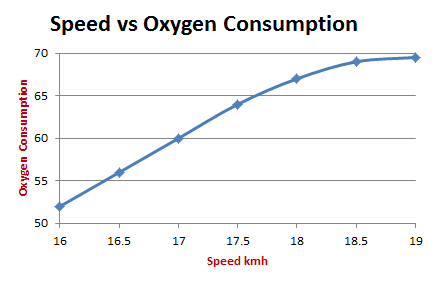
\includegraphics[width=\textwidth]{V02max-running.png}
    \caption{With increasing speed of the runner, oxygen consumption increases linearly and plateaus around 18.5 kilometres per hour - the VO2 max~\cite{vo2max-speed-img}.}
\end{figure}

\subsection*{How to measure Vo2 max}

\subsubsection*{Laboratory test}

Typically, VO2 max is measured directly in laboratory conditions while wearing a respiratory mask, by analyzing inspired and expired breathing gases during maximal exertion~\cite{vo2max-definition}, usually running on a treadmill or riding a stationary bike.

This method of determining VO2 max is highly accurate, but given the need for expensive equipment and trained staff, laboratory testing just isn't feasible for everyday population-wide testing.
On the other hand, results from laboratory tests are often used as reference values for determining the accuracy of alternative methods.

\subsubsection*{Cooper test - Twelve-Minute Run-Walk}

First suggested in the 1970's, Cooper's Twelve-Minute Run-Walk is an endurance test, where the main goal is to run (or walk) as long a distance as possible in twelve minutes.
It was originally developed mainly for armies and police agencies, but it's also popularly (and unnecessarily~\cite{cooper-pupils}) used in schools on untrained pupils.
It is inaccurate for people who do not train running and swim or bike instead, as their bodies are used to a completely different set of movements.

There is a high correlation between the distance an individual can run and their VO2 max value, which can be calculated thusly:

$VO2max = (22.351 \times distance\_in\_kilometers) - 11.288$~\cite{cooper-vo2max}.

\subsubsection*{Multistage Fitness Test - Beep test}

Introduced by a Canadian sports scientist Luc Léger in the 1970s, this aerobic test has consistently been found a reliable way of finding a person's VO2 max.

The original version of the beep test (the Track Test) had the participants running back and forth in the interval of two minutes while the running pace was increased, so they always had to run further than in the previous iteration.

This test was highly efficient, however, given the long intervals and spatial requirements, it couldn't be performed indoors, giving rise to modifications, such as the Twenty-Metre Shuttle Run Test.
As the name suggests, two markers are placed twenty metres apart and again, the participants run back and forth between them, trying to reach the opposite marker before the next -- shorter -- stage begins, that is, before the next beep.
Once the test subject fails to reach a marker, turns without touching the marked line, or starts running before the signal, after one warning, their test is over.
They can also choose to stop when they have reached their maximum physical limit.

The test is divided into stages with recommended running speeds, each stage consisting of multiple shuttles - see the table at~\cite{beep-test-scoring-table}.
From the stage and shuttle reached, one can calculate the VO2 max using the formula

\[VO2max (\frac{ml}{kg*min-1}) = 31.025 + 3.238X - 3.248A + 0.1536AX\]

where $A$ is age of the participant and $X$ is the speed in the final shuttle.
This formula fits the commonly used version of the Beep test (starting at 8.0 km/h, jumping to 9.0 km/h and continuing to rise by 0.5 km/h per level) and may vary depending on the version used~\cite{beep-test-versions}~\cite{beep-test-20m-valid}.

This modified version (just like the original) has been recognized as a valid method to determine VO2 max of male and female adults, individually or in groups, on most gymnasium surfaces~\cite{beep-test-20m-valid}.

In 2017, Tomkinson et al. published a complex systematic study of nearly 1.2 million 9-17 years old children from 50 countries with data from beep tests as old as 1981,
setting standardized norms for testing of fitness in the world's youth~\cite{beep-test-youth-large-study}.


\subsubsection*{Six-Minute Walk Test}

There are also some non-running tests which can be used to measure an individual's VO2 max.

The Six-Minute Walk Test, or 6MWT for short, originated from the Cooper test in the 1980's as a more feasible and less exhausting alternative~\cite{6mwt-history}.

The main objective is for the participant to walk as long a distance as they can in the provided six minutes on a 15- or 30-metre long track, making sharp turns at the end.
Mänttäri et al. published a study in 2018~\cite{6min-walk-test-mantarri}, aimed to develop a prediction model for VO2 max based on 6MWT results combined with heart rate at the end of the 6MWT and easy-to-measure anthropometric and demographic data (such as weight, height, age and gender).
The different track lengths only showed negligible differences between distances walked (on average, 23.5 m longer on the 30-m course).
\textit{For men, the best predictors for VO2max were walking distance, age, BMI, heart rate at the end of 6MWT and height, and for women, walking distance, age and weight} -- surprisingly, heart rate wasn't a significant factor for the female participants.

The formula they developed for men:

 $VO2 max=110.546 + 0.062\times distance - 0.25\times age - 0.486\times BMI - 0.42\times height - 0.109\times HR$

 and for women:

 $VO2 max=22.506 - 0.271\times weight + 0.051\times distance - 0.065\times age$

 \textit{where $weight$ is body weight (kg), $distance$ is distance walked in 6 min (m), $age$ (years), $BMI$ is calculated body mass index (kg/m2), $height$ is body height (cm) and $HR$ is heart rate at the end of the walking test (bpm).}

The authors themselves conclude that their output should be cross-validated with new independent samples of the adult population,
but they consider it a precise enough method to be used for public health monitoring in adults.

Another study from 2015~\cite{6min-walk-test-burr} instead used resting heart rate and arrived at this formula:

$VO2 max =70.161 + 0.023 \times distance - 0.276 \times weight - 6.79 \times sex - 0.193 \times resting_HR - 0.191 \times age$

using $distance$ walked during 6MWT (m), $weight$ (kg), $sex$ -- 1 for female, 0 for male, and $resting_HR$ for resting heart rate in beats per minute.

\subsubsection*{Sit-to-Stand test}

Another test that doesn't require much in terms of space or equipment and is in fact a common daily activity, which is often used to test lower body strength and endurance in older adults, has been studied for correlation with VO2 max values.
The Sit-to-Stand test, which consists of repetitive sitting down and standing up, has acquired a number of different forms just like most other tests used by the general public.
The versions include but aren't limited to the incremental twelve-minute STS test -- sit and stand in incrementally shorter periods of time, repeated for twelve minutes, often controlled by a metronome~\cite{seat-height-sit-to-stand};

Having been closely studied by Nakamura et al., it is a potentially valid test (when done with arm support, to increase the complete exhaustion threshold, and the right chair height, among other factors), but more research needs to be carried out to find a suitable version~\cite{frequencies-sit-to-stand}~\cite{validity-sit-to-stand}.

\subsubsection*{Non-exercise tests}

There are also some tests that do not require exercise and instead, have the individual fill out a questionnaire, such as the Jackson test~\cite{nonexercise-vo2max-test-jackson} or the George test~\cite{nonexercise-vo2max-test-george},
which ask questions on the topic of an individual's exercise habits, such as their perceived level of activity over the last six months.
Every answer has a specific weight in the resulting equation, based on which the person's fitness is evaluated.

These tests, however, should not be used as a sole source of information especially in medicine, as the data is self-reported and may be influenced by bias or conscious falsehood.

\section{The Performance Condition}

A person's VO2 max is recognized as their baseline fitness level index, however, everybody has days when they perform better, and days when they perform worse, while the factors in play are the amount of sleep they get, being sore from previous workouts, and general physical and mental wellbeing.

That is why Firstbeat introduced the Performance Condition.

Firstbeat is a provider of physiological analytics for sports and well-being who have translated human physiology into mathematical models based on heart rate variability (see below).
They provide their analytics engine as a service to a number of fitness device manufacturers, such as Garmin, Xiaomi, Honor and others.

The Performance Condition is a real-time index of a user's immediate fitness and fatigue level compared to their baseline fitness level.

This indicator is measured on a scale of -20 to +20, with each point representing roughly 1\% of their Vo2 max.
So if the user's current Performance Condition is +4, they can expect to perform outstandingly,
but at the same time, during the course of a workout, this number will decrease as fatigue from the exercise gets closer~\cite{performance-condition-firstbeat}~\cite{performance-condition-garmin}.

According to Firstbeat's support personnel, the formula behind the Performance Condition is protected information,
but generally, it uses a combination of personal background data, internal and external workload data, and special guidance from the Firstbeat analytics engine~\cite{firstbeat-performance-condition-emails}.
Garmin's support website provides similar information: it is calculated based on the user's pace, heart rate and heart rate variability (HRV)~\cite{performance-condition-garmin}.

HRV is the variability in intervals between cardiac cycles.
It can be demonstrated, for example, by feeling one's pulse on the wrist while resting and breathing deeply - the interval shortens (heart beating faster) when breathing in, and lengthens (heart beating slower) when breathing out~\cite{hrv}.
It's a complicated enough metric that to calculate it accurately, HRV should be measured using a chest strap,
an intrusive heart rate monitoring method which generally isn't available to a runner on a daily basis.

Additionally, the only activities that are currently supported for determining the Performance Condition, are running and cycling,
and the methods Firstbeat has developed to measure it has failed to satisfy a number of users, leading to them not paying much attention to the metric or outright ignoring the values~\cite{performance-condition-unreliable1}~\cite{performance-condition-unreliable-reasoning}.
One of the reasons behind their dissatisfaction is the fact that the metric only connects the effort the user is making with the distance they are covering,
without taking into account the steepness of the slope, the humidity, temperature, and other external factors 
and should be perceived more as an indicator of simply how much effort your body is making (as explained in BHerman's comment on a post~\cite{performance-condition-unreliable-reasoning} in Firstbeat's forum), 
while being marketed as a highly precise metric that shows you how your training is going and not really explained well to the users.

\section{Heart rate zones}

Everybody has a resting heart rate (for example, right after waking up from a good night's sleep), and a maximum heart rate (the highest number of beats per minute achievable).
The range between HR min and HR max is commonly divided into five zones, based on the effort necessary and the effects the heart rate induces in a person:
\begin{itemize}
    \item Zone 1 (Warm-up and very light exercise) --
    The trainee is relaxed at an easy pace and breathes rhythmically. Keeping one's heart rate in this zone helps with recovery from previous activities.
    \item Zone 2 (Easy, light exercise) --
    The trainee exercises at a comfortable pace, is able to hold a conversation and breathes slightly deeper. This zone is good for endurance practice.
    \item Zone 3 (Aerobic, moderate exercise) --
    At a moderate pace, it is more difficult to hold a conversation. Training in this zone helps improve aerobic capacity.
    \item Zone 4 (Threshold, hard exercise) --
    Training at a fast pace is somewhat uncomfortable, the trainee breathes forcefully. This zone is good for improving speed.
    \item Zone 5 (Maximum) --
    The trainee is at a sprinting pace, which is unsustainable for long period of time, and their breathing is laboured.
    This zone helps increase power in the trainee's body~\cite{garmin-heart-zones}~\cite{polar-heart-zones}.
\end{itemize}

Calculating HR min is an easy enough task - just measure your heart rate right after enjoying some good sleep; HR max is trickier.

\subsection*{Running methods to calculate HR max}
There are some methods to get HR max by running, such as running towards a hill at a high intensity and then ascending the hill at as high intensity as possible,
or, on flat ground, running 400 metres at high intensity and then increasing the intensity for another 400 metres.
These tests are considered stress tests, and individuals who are not highly active are not advised to take them~\cite{hrmax-running-tests}.
Another method is based on interval running:
two intervals, four minutes each, in which the trainee is short of breath, interspersed by three minutes of active rest, and finished by a third interval, where two minutes in the trainee increases their speed as much as they can and run for as long as they can.
HR max is the maximum heart rate achieved~\cite{hrmax-running-tests-intervals}.

\subsection*{Age-based methods to calculate HR max}
As the running methods are generally too difficult to do `on the spot', there have been attempts to calculate HR max based on readily available data.

The most commonly used formula to get one's maximal heart rate,\linebreak $HRmax=220-age$ also known as the Fox formula, has been time and time again found largely inaccurate.
Originally intended as a rough formulation, with cross-sectional data from participants who are by no means representatives of a population~\cite{220-hrmax-new-formula} and based on unoriginal research~\cite{220-hrmax-disproved},
a number of researchers have tried to find similarly simple but more accurate formulas, most of them claiming to have found the right one.
One of the popularly used is the cross-sectional research of Tanaka et al., who formulated the equation $208-0.7\times age$.
This formula was later validated by Gellish et al. in 2007 by conducting an analysis of longitudinal data from participants from various groups and developing a similar formula $207-0.7\times age$,
however, both Fox and Tanaka were disproved by Sarzynski et al. in 2014 as not precise enough based on standard error of estimate (12.4 and 11.4 bpm respectively) of the two formulas~\cite{hrmax-age-disproved}.
In that study, Sarzynski stresses \textit{the importance of finding and validating other measures to be used in exercise prescriptions for the determination of intensity of exercise, the estimation of fitness levels, and as a criterion for achieving maximal exertion.}

The HUNT fitness study carried out on over three thousand people by Nes et al. found a more accurate formula $211-0.64\times age$, with the standard error of estimate of 10.8 bpm, but couldn't find evidence of interaction with gender, physical activity, VO2 max or BMI~\cite{hrmax-Nes-HUNT}.


It seems that computational models for peoples' fitness leave a lot to be desired,
but this can all be remedied with further research.

\chapter{Architecture}
\linebreak
In this chapter I aim to describe the proposed architecture of the solution, starting with a high-level glance -- the component diagram.

The smart wearable gadget will require an application to propagate the data from the heart rate sensor to the smart phone application.
Once the raw data is received, it is combined with GPS data and forwarded through the 'biometric and GPS raw data exchange' interface to the IoT platform, where it gets processed and saved.
When the smart phone application requires it, it requests the processed data through the 'processed data retrieval' and displays it.

\begin{figure}[h]
    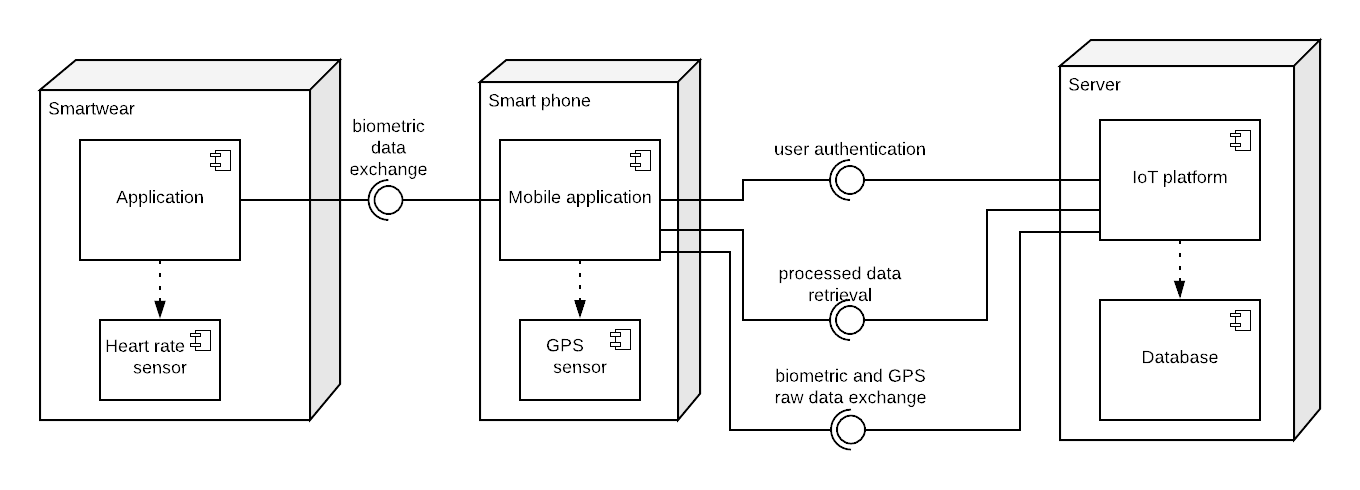
\includegraphics[width=\textwidth]{component.png}
    \caption{Component diagram of the designed IoT solution}
\end{figure}

\setsecnumdepth{part}
\chapter{Conclusion}
\linebreak
For now, I have been spending time mostly thinking about the importance of different features, evaluating the costs of having some compared to others, and how the use cases of existing apps apply to mine.
I have also thought out a high-level architectural model for communication between the components.

\bibliographystyle{iso690}
\bibliography{mybibliographyfile}

\setsecnumdepth{all}
\appendix

\chapter{Acronyms}
\begin{description}
	\item[IoT] Internet of Things -- \textit{The interconnection via the Internet of computing devices embedded in everyday objects, enabling them to send and receive data} \cite{IoT-dictionary} without requiring human-to-human or human-to-computer interaction. \cite{IoT-definition-no-interaction}
	\item[PoC] Proof of Concept -- \textit{Evidence, typically deriving from an experiment or pilot project, which demonstrates that a design concept, business proposal, etc. is feasible.} \cite{PoC-dictionary}
\end{description}


% \chapter{Contents of enclosed CD}

%change appropriately

% \begin{figure}
% 	\dirtree{%
% 		.1 readme.txt\DTcomment{the file with CD contents description}.
% 		.1 exe\DTcomment{the directory with executables}.
% 		.1 src\DTcomment{the directory of source codes}.
% 		.2 wbdcm\DTcomment{implementation sources}.
% 		.2 thesis\DTcomment{the directory of \LaTeX{} source codes of the thesis}.
% 		.1 text\DTcomment{the thesis text directory}.
% 		.2 thesis.pdf\DTcomment{the thesis text in PDF format}.
% 		.2 thesis.ps\DTcomment{the thesis text in PS format}.
% 	}
% \end{figure}

\end{document}
